  % You may change chapter image at will.
% Using 
\chapterbackground{img/dunj.png}
\chapter{Introduction}
\section{Forewords}
This small dungeon is only intended to be an example of use of this OSE class.
There is not intent of quality (nor has it been tested).

It also constitutes an experimentation of \textbf{uncreative dungeon} design using \href{https://chat.openai.com}{ChatGPT}.
All choices described hereafter are from this AI or picked randomly when ChatGPT made several proposition.

%% trick to begin on next column
\vfill
\pagebreak
% long section names can be cut and be unaesthetic..
\section{Introducing the dungeon}
% Use the highlight environment to.. well highlight things
\begin{highlight}[The journey begins] % optional title
  As you make your way through the dense forest, you notice an unusual structure hidden among the trees. 
  It's a small cave, made of rough-hewn stone and nestled into the earth. 
  The entrance is dark and foreboding, but you sense that there is something valuable hidden inside.
  
  As you approach the entrance, you see that the doorway is covered in strange markings and symbols. 
  They seem to pulse with an otherworldly energy, and you feel a sense of unease wash over you. 
  But your curiosity gets the better of you, and you step inside.
  
  The air inside the dungeon is thick and musty, and the darkness is oppressive. 
  You can barely see your hand in front of your face, but you can hear strange noises echoing through the darkness.
  You sense that this place was once used for something sinister.
\end{highlight}

\subsection{Location}
This dungeon may be located within any \emph{"dense forest"}.

This dungeon belongs to ancient ruins :
the forest has grown up around the ruins of an ancient civilization.

\subsection{Rumors}
\begin{enumerate}
  \item The dungeon holds a \textbf{powerful artifact}, guarded by monsters and traps.
  \item The dungeon was built by a \textbf{death-obsessed wizard} who experimented on the living and dead.
  \item A \textbf{secret society} once used the dungeon as a meeting place.
  \item The dungeon is \textbf{cursed} and those who enter never return.
  \item The dungeon is \textbf{haunted by the ghosts} of its unjustly imprisoned former occupants.
  \item A \textbf{powerful demon} is trapped within the dungeon, seeking a way to escape.
\end{enumerate}

\subsection{Hooks}
Here follow a few potential hooks that could lead adventurers to explore the dungeon. 
The Dungeon Master should adapt or customize these hooks to fit the specific needs of their campaign.

\begin{itemize}
  \item A wealthy noble or collector has put out a call for adventurers to \textbf{retrieve a specific artifact} rumored to be located in the dungeon.
  The noble is willing to pay handsomely for its retrieval.
  \item A local village has been plagued by a \textbf{series of mysterious disappearances}, and rumors suggest that the dungeon might be connected to them.
  \item A mysterious stranger offers to sell the adventurers \textbf{an old map} that leads to the dungeon.
  They claim it is the key to a great treasure, but can't enter the dungeon themselves.
  \item A powerful wizard or cleric has sensed a \textbf{disturbance in the magical energies} of the area and believes that the dungeon might be the source. 
  The adventurers are hired to investigate and put an end to the disturbance.
  \item A group of treasure hunters has entered the dungeon and not returned. 
  The adventurers might be hired to \textbf{rescue} them or to retrieve any treasure they left behind.
  \item A local sage or historian has uncovered a lost manuscript that suggests the dungeon contains valuable \textbf{historical or magical knowledge}. 
  The adventurers might be hired to retrieve the manuscript or to explore the dungeon for themselves
\end{itemize}

%% from https://hotpot.ai then upscaled using https://imgupscaler.com/
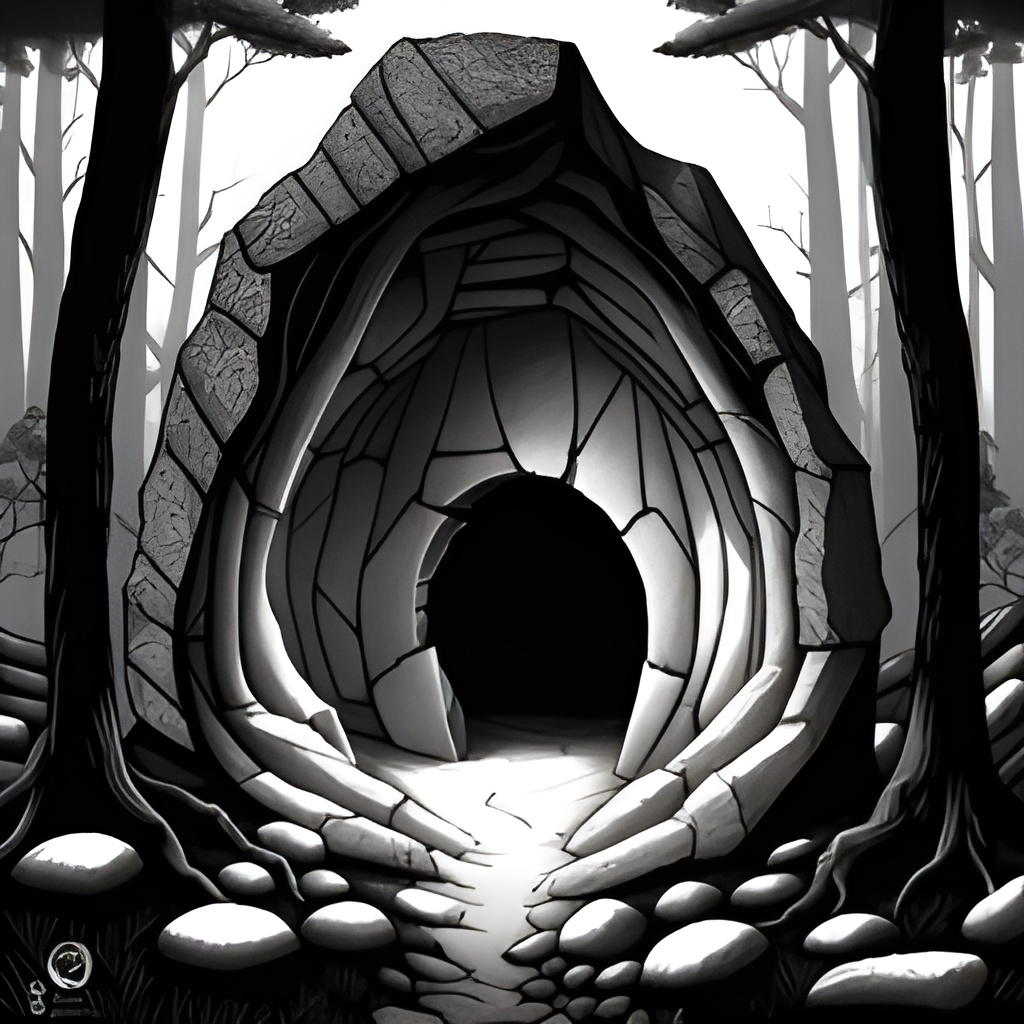
\includegraphics[width=\linewidth]{pics/entrance.jpg}